% Options for packages loaded elsewhere
\PassOptionsToPackage{unicode}{hyperref}
\PassOptionsToPackage{hyphens}{url}
%
\documentclass[
]{article}
\usepackage{lmodern}
\usepackage{amssymb,amsmath}
\usepackage{ifxetex,ifluatex}
\ifnum 0\ifxetex 1\fi\ifluatex 1\fi=0 % if pdftex
  \usepackage[T1]{fontenc}
  \usepackage[utf8]{inputenc}
  \usepackage{textcomp} % provide euro and other symbols
\else % if luatex or xetex
  \usepackage{unicode-math}
  \defaultfontfeatures{Scale=MatchLowercase}
  \defaultfontfeatures[\rmfamily]{Ligatures=TeX,Scale=1}
\fi
% Use upquote if available, for straight quotes in verbatim environments
\IfFileExists{upquote.sty}{\usepackage{upquote}}{}
\IfFileExists{microtype.sty}{% use microtype if available
  \usepackage[]{microtype}
  \UseMicrotypeSet[protrusion]{basicmath} % disable protrusion for tt fonts
}{}
\makeatletter
\@ifundefined{KOMAClassName}{% if non-KOMA class
  \IfFileExists{parskip.sty}{%
    \usepackage{parskip}
  }{% else
    \setlength{\parindent}{0pt}
    \setlength{\parskip}{6pt plus 2pt minus 1pt}}
}{% if KOMA class
  \KOMAoptions{parskip=half}}
\makeatother
\usepackage{xcolor}
\IfFileExists{xurl.sty}{\usepackage{xurl}}{} % add URL line breaks if available
\IfFileExists{bookmark.sty}{\usepackage{bookmark}}{\usepackage{hyperref}}
\hypersetup{
  pdftitle={Statistical Learning Project - Unsupervised Learning},
  hidelinks,
  pdfcreator={LaTeX via pandoc}}
\urlstyle{same} % disable monospaced font for URLs
\usepackage[margin=1in]{geometry}
\usepackage{color}
\usepackage{fancyvrb}
\newcommand{\VerbBar}{|}
\newcommand{\VERB}{\Verb[commandchars=\\\{\}]}
\DefineVerbatimEnvironment{Highlighting}{Verbatim}{commandchars=\\\{\}}
% Add ',fontsize=\small' for more characters per line
\usepackage{framed}
\definecolor{shadecolor}{RGB}{248,248,248}
\newenvironment{Shaded}{\begin{snugshade}}{\end{snugshade}}
\newcommand{\AlertTok}[1]{\textcolor[rgb]{0.94,0.16,0.16}{#1}}
\newcommand{\AnnotationTok}[1]{\textcolor[rgb]{0.56,0.35,0.01}{\textbf{\textit{#1}}}}
\newcommand{\AttributeTok}[1]{\textcolor[rgb]{0.77,0.63,0.00}{#1}}
\newcommand{\BaseNTok}[1]{\textcolor[rgb]{0.00,0.00,0.81}{#1}}
\newcommand{\BuiltInTok}[1]{#1}
\newcommand{\CharTok}[1]{\textcolor[rgb]{0.31,0.60,0.02}{#1}}
\newcommand{\CommentTok}[1]{\textcolor[rgb]{0.56,0.35,0.01}{\textit{#1}}}
\newcommand{\CommentVarTok}[1]{\textcolor[rgb]{0.56,0.35,0.01}{\textbf{\textit{#1}}}}
\newcommand{\ConstantTok}[1]{\textcolor[rgb]{0.00,0.00,0.00}{#1}}
\newcommand{\ControlFlowTok}[1]{\textcolor[rgb]{0.13,0.29,0.53}{\textbf{#1}}}
\newcommand{\DataTypeTok}[1]{\textcolor[rgb]{0.13,0.29,0.53}{#1}}
\newcommand{\DecValTok}[1]{\textcolor[rgb]{0.00,0.00,0.81}{#1}}
\newcommand{\DocumentationTok}[1]{\textcolor[rgb]{0.56,0.35,0.01}{\textbf{\textit{#1}}}}
\newcommand{\ErrorTok}[1]{\textcolor[rgb]{0.64,0.00,0.00}{\textbf{#1}}}
\newcommand{\ExtensionTok}[1]{#1}
\newcommand{\FloatTok}[1]{\textcolor[rgb]{0.00,0.00,0.81}{#1}}
\newcommand{\FunctionTok}[1]{\textcolor[rgb]{0.00,0.00,0.00}{#1}}
\newcommand{\ImportTok}[1]{#1}
\newcommand{\InformationTok}[1]{\textcolor[rgb]{0.56,0.35,0.01}{\textbf{\textit{#1}}}}
\newcommand{\KeywordTok}[1]{\textcolor[rgb]{0.13,0.29,0.53}{\textbf{#1}}}
\newcommand{\NormalTok}[1]{#1}
\newcommand{\OperatorTok}[1]{\textcolor[rgb]{0.81,0.36,0.00}{\textbf{#1}}}
\newcommand{\OtherTok}[1]{\textcolor[rgb]{0.56,0.35,0.01}{#1}}
\newcommand{\PreprocessorTok}[1]{\textcolor[rgb]{0.56,0.35,0.01}{\textit{#1}}}
\newcommand{\RegionMarkerTok}[1]{#1}
\newcommand{\SpecialCharTok}[1]{\textcolor[rgb]{0.00,0.00,0.00}{#1}}
\newcommand{\SpecialStringTok}[1]{\textcolor[rgb]{0.31,0.60,0.02}{#1}}
\newcommand{\StringTok}[1]{\textcolor[rgb]{0.31,0.60,0.02}{#1}}
\newcommand{\VariableTok}[1]{\textcolor[rgb]{0.00,0.00,0.00}{#1}}
\newcommand{\VerbatimStringTok}[1]{\textcolor[rgb]{0.31,0.60,0.02}{#1}}
\newcommand{\WarningTok}[1]{\textcolor[rgb]{0.56,0.35,0.01}{\textbf{\textit{#1}}}}
\usepackage{graphicx,grffile}
\makeatletter
\def\maxwidth{\ifdim\Gin@nat@width>\linewidth\linewidth\else\Gin@nat@width\fi}
\def\maxheight{\ifdim\Gin@nat@height>\textheight\textheight\else\Gin@nat@height\fi}
\makeatother
% Scale images if necessary, so that they will not overflow the page
% margins by default, and it is still possible to overwrite the defaults
% using explicit options in \includegraphics[width, height, ...]{}
\setkeys{Gin}{width=\maxwidth,height=\maxheight,keepaspectratio}
% Set default figure placement to htbp
\makeatletter
\def\fps@figure{htbp}
\makeatother
\setlength{\emergencystretch}{3em} % prevent overfull lines
\providecommand{\tightlist}{%
  \setlength{\itemsep}{0pt}\setlength{\parskip}{0pt}}
\setcounter{secnumdepth}{-\maxdimen} % remove section numbering

\title{Statistical Learning Project - Unsupervised Learning}
\author{}
\date{\vspace{-2.5em}}

\begin{document}
\maketitle

\begin{Shaded}
\begin{Highlighting}[]
\CommentTok{#https://www.kaggle.com/dgomonov/new-york-city-airbnb-open-data}
\KeywordTok{library}\NormalTok{(ggplot2)}
\end{Highlighting}
\end{Shaded}

\begin{verbatim}
## Warning: package 'ggplot2' was built under R version 3.6.3
\end{verbatim}

\begin{Shaded}
\begin{Highlighting}[]
\KeywordTok{library}\NormalTok{(ggmap)}
\end{Highlighting}
\end{Shaded}

\begin{verbatim}
## Warning: package 'ggmap' was built under R version 3.6.3
\end{verbatim}

\begin{verbatim}
## Google's Terms of Service: https://cloud.google.com/maps-platform/terms/.
\end{verbatim}

\begin{verbatim}
## Please cite ggmap if you use it! See citation("ggmap") for details.
\end{verbatim}

\begin{Shaded}
\begin{Highlighting}[]
\KeywordTok{library}\NormalTok{(tidyr)}
\KeywordTok{library}\NormalTok{(cowplot)}
\end{Highlighting}
\end{Shaded}

\begin{verbatim}
## Warning: package 'cowplot' was built under R version 3.6.3
\end{verbatim}

\begin{verbatim}
## 
## ********************************************************
\end{verbatim}

\begin{verbatim}
## Note: As of version 1.0.0, cowplot does not change the
\end{verbatim}

\begin{verbatim}
##   default ggplot2 theme anymore. To recover the previous
\end{verbatim}

\begin{verbatim}
##   behavior, execute:
##   theme_set(theme_cowplot())
\end{verbatim}

\begin{verbatim}
## ********************************************************
\end{verbatim}

\begin{verbatim}
## 
## Attaching package: 'cowplot'
\end{verbatim}

\begin{verbatim}
## The following object is masked from 'package:ggmap':
## 
##     theme_nothing
\end{verbatim}

\begin{Shaded}
\begin{Highlighting}[]
\KeywordTok{library}\NormalTok{(magick)}
\end{Highlighting}
\end{Shaded}

\begin{verbatim}
## Warning: package 'magick' was built under R version 3.6.3
\end{verbatim}

\begin{verbatim}
## Linking to ImageMagick 6.9.9.14
## Enabled features: cairo, freetype, fftw, ghostscript, lcms, pango, rsvg, webp
## Disabled features: fontconfig, x11
\end{verbatim}

\begin{Shaded}
\begin{Highlighting}[]
\KeywordTok{library}\NormalTok{(dplyr)}
\end{Highlighting}
\end{Shaded}

\begin{verbatim}
## Warning: package 'dplyr' was built under R version 3.6.3
\end{verbatim}

\begin{verbatim}
## 
## Attaching package: 'dplyr'
\end{verbatim}

\begin{verbatim}
## The following objects are masked from 'package:stats':
## 
##     filter, lag
\end{verbatim}

\begin{verbatim}
## The following objects are masked from 'package:base':
## 
##     intersect, setdiff, setequal, union
\end{verbatim}

\begin{Shaded}
\begin{Highlighting}[]
\CommentTok{#world_map <- map_data("newyork")}
\end{Highlighting}
\end{Shaded}

\hypertarget{read-dataset}{%
\section{Read Dataset}\label{read-dataset}}

\begin{Shaded}
\begin{Highlighting}[]
\NormalTok{ds =}\StringTok{ }\KeywordTok{read.csv}\NormalTok{(}\StringTok{"AB_NYC_2019.csv"}\NormalTok{)}
\KeywordTok{head}\NormalTok{(ds)}
\end{Highlighting}
\end{Shaded}

\begin{verbatim}
##     id                                             name host_id   host_name
## 1 2539               Clean & quiet apt home by the park    2787        John
## 2 2595                            Skylit Midtown Castle    2845    Jennifer
## 3 3647              THE VILLAGE OF HARLEM....NEW YORK !    4632   Elisabeth
## 4 3831                  Cozy Entire Floor of Brownstone    4869 LisaRoxanne
## 5 5022 Entire Apt: Spacious Studio/Loft by central park    7192       Laura
## 6 5099        Large Cozy 1 BR Apartment In Midtown East    7322       Chris
##   neighbourhood_group neighbourhood latitude longitude       room_type price
## 1            Brooklyn    Kensington 40.64749 -73.97237    Private room   149
## 2           Manhattan       Midtown 40.75362 -73.98377 Entire home/apt   225
## 3           Manhattan        Harlem 40.80902 -73.94190    Private room   150
## 4            Brooklyn  Clinton Hill 40.68514 -73.95976 Entire home/apt    89
## 5           Manhattan   East Harlem 40.79851 -73.94399 Entire home/apt    80
## 6           Manhattan   Murray Hill 40.74767 -73.97500 Entire home/apt   200
##   minimum_nights number_of_reviews last_review reviews_per_month
## 1              1                 9  2018-10-19              0.21
## 2              1                45  2019-05-21              0.38
## 3              3                 0                            NA
## 4              1               270  2019-07-05              4.64
## 5             10                 9  2018-11-19              0.10
## 6              3                74  2019-06-22              0.59
##   calculated_host_listings_count availability_365
## 1                              6              365
## 2                              2              355
## 3                              1              365
## 4                              1              194
## 5                              1                0
## 6                              1              129
\end{verbatim}

\hypertarget{data-cleaning}{%
\section{Data cleaning}\label{data-cleaning}}

\hypertarget{check-for-na-and-null-values}{%
\subsection{Check for NA and NULL
values}\label{check-for-na-and-null-values}}

\begin{Shaded}
\begin{Highlighting}[]
\CommentTok{#Check for NA}
\KeywordTok{apply}\NormalTok{(ds,}\DecValTok{2}\NormalTok{,}\ControlFlowTok{function}\NormalTok{(x) }\KeywordTok{sum}\NormalTok{(}\KeywordTok{is.na}\NormalTok{(x)))}
\end{Highlighting}
\end{Shaded}

\begin{verbatim}
##                             id                           name 
##                              0                              0 
##                        host_id                      host_name 
##                              0                              0 
##            neighbourhood_group                  neighbourhood 
##                              0                              0 
##                       latitude                      longitude 
##                              0                              0 
##                      room_type                          price 
##                              0                              0 
##                 minimum_nights              number_of_reviews 
##                              0                              0 
##                    last_review              reviews_per_month 
##                              0                          10052 
## calculated_host_listings_count               availability_365 
##                              0                              0
\end{verbatim}

\begin{Shaded}
\begin{Highlighting}[]
\CommentTok{# NOTES}
\CommentTok{# Remove NA, empty}
\CommentTok{#}
\CommentTok{#}
\CommentTok{#}
\CommentTok{#}
\end{Highlighting}
\end{Shaded}

\hypertarget{normalisation-and-selection-of-the-variables}{%
\subsection{Normalisation and selection of the
variables}\label{normalisation-and-selection-of-the-variables}}

\begin{Shaded}
\begin{Highlighting}[]
\NormalTok{normalize <-}\StringTok{ }\ControlFlowTok{function}\NormalTok{(x) \{}
  \KeywordTok{return}\NormalTok{ ((x }\OperatorTok{-}\StringTok{ }\KeywordTok{min}\NormalTok{(x)) }\OperatorTok{/}\StringTok{ }\NormalTok{(}\KeywordTok{max}\NormalTok{(x) }\OperatorTok{-}\StringTok{ }\KeywordTok{min}\NormalTok{(x)))}
\NormalTok{\}}


\NormalTok{clean_data =}\StringTok{ }\ControlFlowTok{function}\NormalTok{(ds)}
\NormalTok{\{}
\NormalTok{  ds =}\StringTok{ }\KeywordTok{select}\NormalTok{ (ds,}\OperatorTok{-}\KeywordTok{c}\NormalTok{(host_id, id, host_name, name,minimum_nights,number_of_reviews,}
\NormalTok{                     neighbourhood,last_review,availability_}\DecValTok{365}\NormalTok{,}
                     
\NormalTok{                     reviews_per_month,calculated_host_listings_count))}
 

\NormalTok{  numerical =}\StringTok{ }\KeywordTok{c}\NormalTok{(}\StringTok{"price"}\NormalTok{,}\StringTok{"longitude"}\NormalTok{, }\StringTok{"latitude"}\NormalTok{)}
\NormalTok{  categorical =}\StringTok{ }\KeywordTok{c}\NormalTok{(}\StringTok{"neighbourhood_group"}\NormalTok{)}
  
\NormalTok{  ds[numerical] =}\StringTok{ }\KeywordTok{scale}\NormalTok{(ds[numerical])}
\NormalTok{  ds}\OperatorTok{$}\NormalTok{neighbourhood_group =}\StringTok{ }\KeywordTok{factor}\NormalTok{(ds}\OperatorTok{$}\NormalTok{neighbourhood_group, }
                                  \DataTypeTok{level=} \KeywordTok{c}\NormalTok{(}\StringTok{"Brooklyn"}\NormalTok{,}\StringTok{"Manhattan"}\NormalTok{,}
                                           \StringTok{"Queens"}\NormalTok{,}\StringTok{"Staten Island"}\NormalTok{, }\StringTok{"Bronx"}\NormalTok{), }
                                  \DataTypeTok{labels=}\KeywordTok{c}\NormalTok{(}\DecValTok{1}\NormalTok{,}\DecValTok{2}\NormalTok{,}\DecValTok{3}\NormalTok{,}\DecValTok{4}\NormalTok{,}\DecValTok{5}\NormalTok{))}
\NormalTok{  ds}\OperatorTok{$}\NormalTok{room_type =}\StringTok{ }\KeywordTok{factor}\NormalTok{(ds}\OperatorTok{$}\NormalTok{room_type, }
                        \DataTypeTok{level=} \KeywordTok{c}\NormalTok{(}\StringTok{"Private room"}\NormalTok{,}\StringTok{"Entire home/apt"}\NormalTok{,}\StringTok{"Shared room"}\NormalTok{), }
                        \DataTypeTok{labels=}\KeywordTok{c}\NormalTok{(}\DecValTok{1}\NormalTok{,}\DecValTok{2}\NormalTok{,}\DecValTok{3}\NormalTok{))}
  
  \KeywordTok{return}\NormalTok{(ds)}
\NormalTok{\}}
\CommentTok{#ggdraw() +}
\CommentTok{#  draw_image("New_York_City_.png") +}
\CommentTok{#  draw_plot(myplot)}

\NormalTok{dataset =}\StringTok{ }\KeywordTok{clean_data}\NormalTok{(ds)}

\KeywordTok{head}\NormalTok{(dataset)}
\end{Highlighting}
\end{Shaded}

\begin{verbatim}
##   neighbourhood_group   latitude  longitude room_type       price
## 1                   1 -1.4938339 -0.4376476         1 -0.01549291
## 2                   2  0.4524314 -0.6846321         2  0.30097047
## 3                   2  1.4683845  0.2224944         1 -0.01132892
## 4                   1 -0.8033893 -0.1644481         2 -0.26533242
## 5                   2  1.2756468  0.1772139         2 -0.30280835
## 6                   2  0.3433173 -0.4946274         2  0.19687067
\end{verbatim}

\hypertarget{k-means}{%
\section{K-MEANS}\label{k-means}}

\textbf{x}: numeric matrix, numeric data frame or a numeric vector
\textbf{centers}: Possible values are the number of clusters (k) or a
set of initial (distinct) cluster centers. If a number, a random set of
(distinct) rows in x is chosen as the initial centers.
\textbf{iter.max}: The maximum number of iterations allowed. Default
value is 10. \textbf{nstart}: The number of random starting partitions
when centers is a number. Trying nstart \textgreater{} 1 is often
recommended.

\begin{Shaded}
\begin{Highlighting}[]
\NormalTok{km.res =}\StringTok{ }\KeywordTok{kmeans}\NormalTok{(dataset, }\DecValTok{4}\NormalTok{, }\DataTypeTok{nstart =} \DecValTok{25}\NormalTok{)}

\KeywordTok{cat}\NormalTok{(}\StringTok{"First 10 Clusters association"}\NormalTok{,km.res}\OperatorTok{$}\NormalTok{cluster[}\DecValTok{1}\OperatorTok{:}\DecValTok{10}\NormalTok{])}
\end{Highlighting}
\end{Shaded}

\begin{verbatim}
## First 10 Clusters association 3 1 1 3 1 1 3 1 1 1
\end{verbatim}

\begin{Shaded}
\begin{Highlighting}[]
\KeywordTok{cat}\NormalTok{(}\StringTok{"}\CharTok{\textbackslash{}n}\StringTok{Centers"}\NormalTok{)}
\end{Highlighting}
\end{Shaded}

\begin{verbatim}
## 
## Centers
\end{verbatim}

\begin{Shaded}
\begin{Highlighting}[]
\KeywordTok{print}\NormalTok{(km.res}\OperatorTok{$}\NormalTok{centers)}
\end{Highlighting}
\end{Shaded}

\begin{verbatim}
##   neighbourhood_group   latitude   longitude room_type      price
## 1            2.051265  0.6141866 -0.51376305  1.650961  0.1253757
## 2            1.868421  0.1287874 -0.50832977  1.824561 14.7620392
## 3            1.002839 -0.8078700  0.01786529  1.515912 -0.1419676
## 4            3.346637  0.3881026  1.78314575  1.427095 -0.2611466
\end{verbatim}

\begin{Shaded}
\begin{Highlighting}[]
\KeywordTok{cat}\NormalTok{(}\StringTok{"}\CharTok{\textbackslash{}n}\StringTok{totss"}\NormalTok{,km.res}\OperatorTok{$}\NormalTok{totss)}
\end{Highlighting}
\end{Shaded}

\begin{verbatim}
## 
## totss 195866.3
\end{verbatim}

\begin{Shaded}
\begin{Highlighting}[]
\KeywordTok{cat}\NormalTok{(}\StringTok{"}\CharTok{\textbackslash{}n}\StringTok{withinss"}\NormalTok{,km.res}\OperatorTok{$}\NormalTok{withinss)}
\end{Highlighting}
\end{Shaded}

\begin{verbatim}
## 
## withinss 39332.74 9312.047 21164.81 22019.68
\end{verbatim}

\begin{Shaded}
\begin{Highlighting}[]
\KeywordTok{cat}\NormalTok{(}\StringTok{"}\CharTok{\textbackslash{}n}\StringTok{tot_withinss"}\NormalTok{,km.res}\OperatorTok{$}\NormalTok{tot.withinss)}
\end{Highlighting}
\end{Shaded}

\begin{verbatim}
## 
## tot_withinss 91829.28
\end{verbatim}

\begin{Shaded}
\begin{Highlighting}[]
\KeywordTok{cat}\NormalTok{(}\StringTok{"}\CharTok{\textbackslash{}n}\StringTok{betweenss"}\NormalTok{,km.res}\OperatorTok{$}\NormalTok{betweenss)}
\end{Highlighting}
\end{Shaded}

\begin{verbatim}
## 
## betweenss 104037.1
\end{verbatim}

\begin{Shaded}
\begin{Highlighting}[]
\KeywordTok{cat}\NormalTok{(}\StringTok{"}\CharTok{\textbackslash{}n}\StringTok{Size"}\NormalTok{,km.res}\OperatorTok{$}\NormalTok{size)}
\end{Highlighting}
\end{Shaded}

\begin{verbatim}
## 
## Size 22413 114 20079 6289
\end{verbatim}

\begin{Shaded}
\begin{Highlighting}[]
\KeywordTok{cat}\NormalTok{(}\StringTok{"}\CharTok{\textbackslash{}n}\StringTok{iter"}\NormalTok{,km.res}\OperatorTok{$}\NormalTok{iter)}
\end{Highlighting}
\end{Shaded}

\begin{verbatim}
## 
## iter 3
\end{verbatim}

\begin{Shaded}
\begin{Highlighting}[]
\KeywordTok{cat}\NormalTok{(}\StringTok{"}\CharTok{\textbackslash{}n}\StringTok{ifault"}\NormalTok{,km.res}\OperatorTok{$}\NormalTok{ifault)}
\end{Highlighting}
\end{Shaded}

\begin{verbatim}
## 
## ifault 0
\end{verbatim}

To create a beautiful graph of the clusters generated with the kmeans()
function, will use the factoextra package.

\begin{Shaded}
\begin{Highlighting}[]
\KeywordTok{library}\NormalTok{(factoextra)}
\end{Highlighting}
\end{Shaded}

\begin{verbatim}
## Warning: package 'factoextra' was built under R version 3.6.3
\end{verbatim}

\begin{verbatim}
## Welcome! Want to learn more? See two factoextra-related books at https://goo.gl/ve3WBa
\end{verbatim}

Cluster number for each of the observations

\begin{Shaded}
\begin{Highlighting}[]
\KeywordTok{head}\NormalTok{(km.res}\OperatorTok{$}\NormalTok{cluster)}
\end{Highlighting}
\end{Shaded}

\begin{verbatim}
## [1] 3 1 1 3 1 1
\end{verbatim}

Cluster size

\begin{Shaded}
\begin{Highlighting}[]
\NormalTok{km.res}\OperatorTok{$}\NormalTok{size}
\end{Highlighting}
\end{Shaded}

\begin{verbatim}
## [1] 22413   114 20079  6289
\end{verbatim}

Cluster means

\begin{Shaded}
\begin{Highlighting}[]
\NormalTok{km.res}\OperatorTok{$}\NormalTok{centers}
\end{Highlighting}
\end{Shaded}

\begin{verbatim}
##   neighbourhood_group   latitude   longitude room_type      price
## 1            2.051265  0.6141866 -0.51376305  1.650961  0.1253757
## 2            1.868421  0.1287874 -0.50832977  1.824561 14.7620392
## 3            1.002839 -0.8078700  0.01786529  1.515912 -0.1419676
## 4            3.346637  0.3881026  1.78314575  1.427095 -0.2611466
\end{verbatim}

\begin{Shaded}
\begin{Highlighting}[]
\CommentTok{#dataset$neighbourhood_group = as.numeric( dataset$neighbourhood_group)}
\CommentTok{#dataset$room_type = as.numeric(  dataset$room_type)}
\CommentTok{#fviz_cluster(km.res, data = dataset,}
\CommentTok{#             palette = c("#00AFBB","#2E9FDF", "#E7B800", "#FC4E07"),}
\CommentTok{#             ggtheme = theme_minimal(),}
\CommentTok{#             main = "Partitioning Clustering Plot"}
\CommentTok{#)}

\CommentTok{#res <- hcut(dataset, k = 4, stand = FALSE)}
\CommentTok{#fviz_dend(km.res, rect = TRUE, cex = 0.5,}
\CommentTok{#          k_colors = c("#00AFBB","#2E9FDF", "#E7B800", "#FC4E07"))}
\end{Highlighting}
\end{Shaded}

\hypertarget{pam-algorithm}{%
\section{PAM ALGORITHM}\label{pam-algorithm}}

\url{https://towardsdatascience.com/clustering-on-mixed-type-data-8bbd0a2569c3}

\begin{Shaded}
\begin{Highlighting}[]
\KeywordTok{library}\NormalTok{(cluster)}
\KeywordTok{library}\NormalTok{(readr)}
\KeywordTok{library}\NormalTok{(Rtsne)}
\end{Highlighting}
\end{Shaded}

\begin{verbatim}
## Warning: package 'Rtsne' was built under R version 3.6.3
\end{verbatim}

Compute Gower distance

\begin{Shaded}
\begin{Highlighting}[]
\KeywordTok{dim}\NormalTok{(dataset)}
\end{Highlighting}
\end{Shaded}

\begin{verbatim}
## [1] 48895     5
\end{verbatim}

\begin{Shaded}
\begin{Highlighting}[]
\NormalTok{smp_size <-}\StringTok{ }\KeywordTok{floor}\NormalTok{(}\FloatTok{0.9} \OperatorTok{*}\StringTok{ }\KeywordTok{nrow}\NormalTok{(dataset))}
\KeywordTok{set.seed}\NormalTok{(}\DecValTok{123}\NormalTok{)}

\NormalTok{train_ind <-}\StringTok{ }\KeywordTok{sample}\NormalTok{(}\KeywordTok{seq_len}\NormalTok{(}\KeywordTok{nrow}\NormalTok{(dataset)), }\DataTypeTok{size =}\NormalTok{ smp_size)}

\NormalTok{prova =}\StringTok{ }\NormalTok{dataset[}\OperatorTok{-}\NormalTok{train_ind,]}
\NormalTok{pam.res <-}\StringTok{ }\KeywordTok{pam}\NormalTok{(prova, }\DecValTok{4}\NormalTok{)}

\NormalTok{gower_dist <-}\StringTok{ }\KeywordTok{daisy}\NormalTok{(prova, }\DataTypeTok{metric =} \StringTok{"gower"}\NormalTok{)}
\end{Highlighting}
\end{Shaded}

\begin{Shaded}
\begin{Highlighting}[]
\NormalTok{start.time <-}\StringTok{ }\KeywordTok{Sys.time}\NormalTok{()}
\NormalTok{sil_width <-}\StringTok{ }\KeywordTok{c}\NormalTok{(}\OtherTok{NA}\NormalTok{)}
\ControlFlowTok{for}\NormalTok{(i }\ControlFlowTok{in} \DecValTok{2}\OperatorTok{:}\DecValTok{8}\NormalTok{)\{  }
\NormalTok{  pam_fit <-}\StringTok{ }\KeywordTok{pam}\NormalTok{(gower_dist, }\DataTypeTok{diss =} \OtherTok{TRUE}\NormalTok{, }\DataTypeTok{k =}\NormalTok{ i)  }
\NormalTok{  sil_width[i] <-}\StringTok{ }\NormalTok{pam_fit}\OperatorTok{$}\NormalTok{silinfo}\OperatorTok{$}\NormalTok{avg.width  }
\NormalTok{\}}


\NormalTok{end.time <-}\StringTok{ }\KeywordTok{Sys.time}\NormalTok{()}
\NormalTok{time.taken <-}\StringTok{ }\NormalTok{end.time }\OperatorTok{-}\StringTok{ }\NormalTok{start.time}

\KeywordTok{print}\NormalTok{(}\StringTok{"-- Time: -- "}\NormalTok{)}
\end{Highlighting}
\end{Shaded}

\begin{verbatim}
## [1] "-- Time: -- "
\end{verbatim}

\begin{Shaded}
\begin{Highlighting}[]
\NormalTok{time.taken}
\end{Highlighting}
\end{Shaded}

\begin{verbatim}
## Time difference of 1.482687 mins
\end{verbatim}

\begin{Shaded}
\begin{Highlighting}[]
\KeywordTok{print}\NormalTok{(}\StringTok{""}\NormalTok{)}
\end{Highlighting}
\end{Shaded}

\begin{verbatim}
## [1] ""
\end{verbatim}

\begin{Shaded}
\begin{Highlighting}[]
\KeywordTok{plot}\NormalTok{(}\DecValTok{1}\OperatorTok{:}\DecValTok{8}\NormalTok{, sil_width,}
      \DataTypeTok{xlab =} \StringTok{"Number of clusters"}\NormalTok{,}
      \DataTypeTok{ylab =} \StringTok{"Silhouette Width"}\NormalTok{)}
\KeywordTok{lines}\NormalTok{(}\DecValTok{1}\OperatorTok{:}\DecValTok{8}\NormalTok{, sil_width)}
\end{Highlighting}
\end{Shaded}

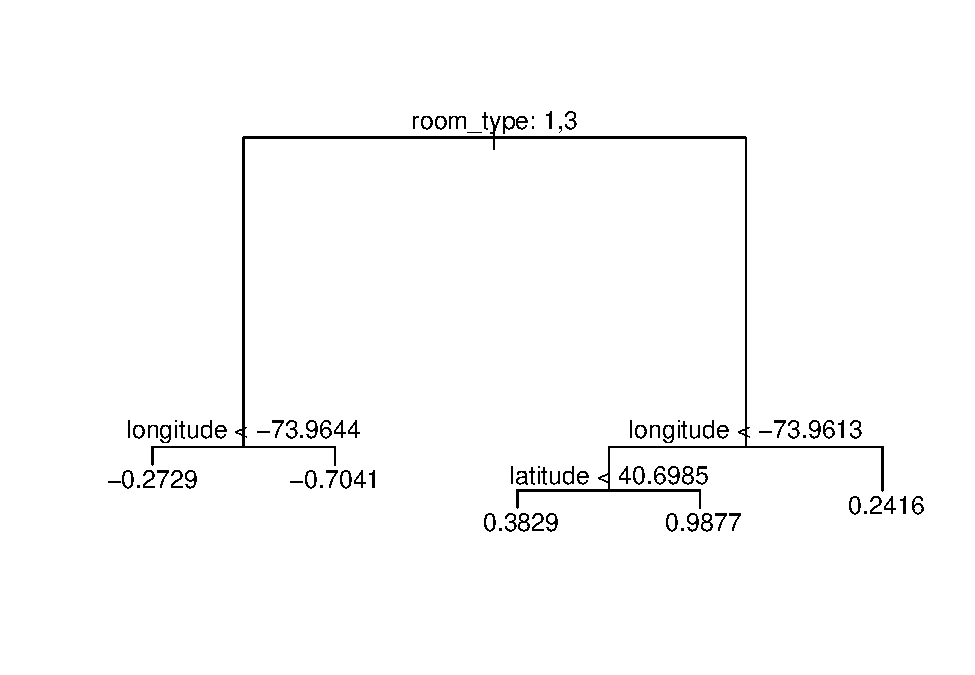
\includegraphics{unsupervised_files/figure-latex/unnamed-chunk-13-1.pdf}

\hypertarget{famd}{%
\section{FAMD}\label{famd}}

\url{http://www.sthda.com/english/articles/31-principal-component-methods-in-r-practical-guide/115-famd-factor-analysis-of-mixed-data-in-r-essentials/}
\url{https://nextjournal.com/pc-methods/calculate-pc-mixed-data}
\url{https://cran.r-project.org/web/packages/FactoMineR/index.html}
\url{https://stats.stackexchange.com/questions/5774/can-principal-component-analysis-be-applied-to-datasets-containing-a-mix-of-cont}

\begin{Shaded}
\begin{Highlighting}[]
\KeywordTok{library}\NormalTok{(}\StringTok{"FactoMineR"}\NormalTok{)}
\end{Highlighting}
\end{Shaded}

\begin{verbatim}
## Warning: package 'FactoMineR' was built under R version 3.6.3
\end{verbatim}

\begin{Shaded}
\begin{Highlighting}[]
\KeywordTok{library}\NormalTok{(}\StringTok{"factoextra"}\NormalTok{)}
\end{Highlighting}
\end{Shaded}

FAMD (base, ncp = 5, sup.var = NULL, ind.sup = NULL, graph = TRUE) -
base : a data frame with n rows (individuals) and p columns (variables).
- ncp: the number of dimensions kept in the results (by default 5) -
sup.var: a vector indicating the indexes of the supplementary variables.
- ind.sup: a vector indicating the indexes of the supplementary
individuals. - graph : a logical value. If TRUE a graph is displayed.

\begin{Shaded}
\begin{Highlighting}[]
\NormalTok{res.famd <-}\StringTok{ }\KeywordTok{FAMD}\NormalTok{(dataset, }\DataTypeTok{graph =} \OtherTok{FALSE}\NormalTok{, }\DataTypeTok{ncp =} \DecValTok{10}\NormalTok{)}
\KeywordTok{print}\NormalTok{(res.famd)}
\end{Highlighting}
\end{Shaded}

\begin{verbatim}
## *The results are available in the following objects:
## 
##   name          description                             
## 1 "$eig"        "eigenvalues and inertia"               
## 2 "$var"        "Results for the variables"             
## 3 "$ind"        "results for the individuals"           
## 4 "$quali.var"  "Results for the qualitative variables" 
## 5 "$quanti.var" "Results for the quantitative variables"
\end{verbatim}

\begin{Shaded}
\begin{Highlighting}[]
\NormalTok{eig.val <-}\StringTok{ }\KeywordTok{get_eigenvalue}\NormalTok{(res.famd)}
\KeywordTok{head}\NormalTok{(eig.val)}
\end{Highlighting}
\end{Shaded}

\begin{verbatim}
##       eigenvalue variance.percent cumulative.variance.percent
## Dim.1  1.9083514         21.20390                    21.20390
## Dim.2  1.7965387         19.96154                    41.16545
## Dim.3  1.1478319         12.75369                    53.91913
## Dim.4  1.0050505         11.16723                    65.08636
## Dim.5  0.9953729         11.05970                    76.14606
## Dim.6  0.9550886         10.61210                    86.75815
\end{verbatim}

\begin{Shaded}
\begin{Highlighting}[]
\KeywordTok{fviz_screeplot}\NormalTok{(res.famd)}
\end{Highlighting}
\end{Shaded}

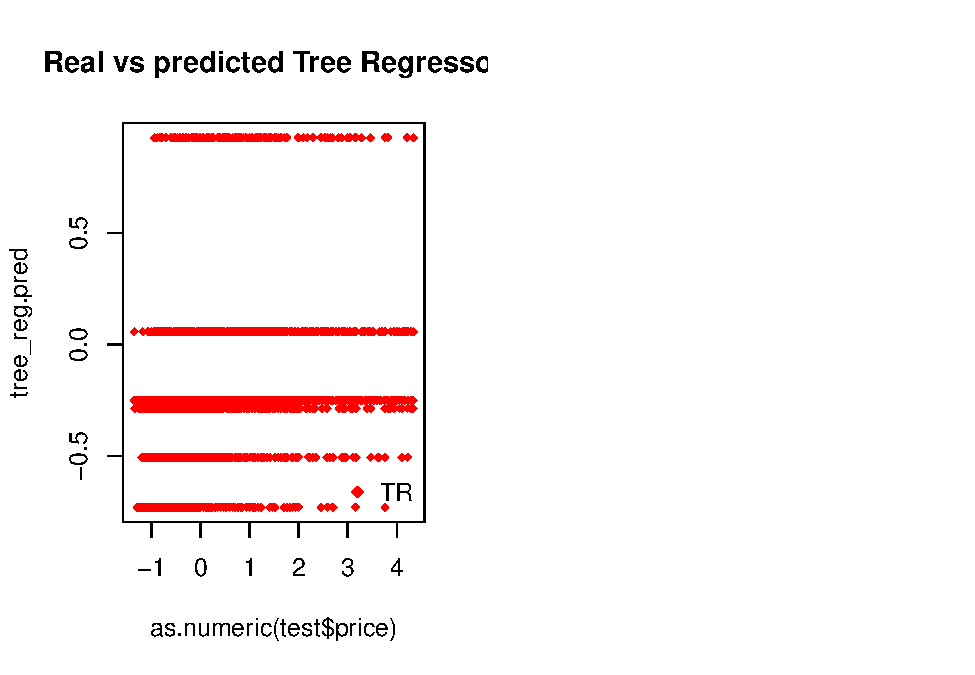
\includegraphics{unsupervised_files/figure-latex/unnamed-chunk-16-1.pdf}

\begin{Shaded}
\begin{Highlighting}[]
\NormalTok{var <-}\StringTok{ }\KeywordTok{get_famd_var}\NormalTok{(res.famd)}
\NormalTok{var}
\end{Highlighting}
\end{Shaded}

\begin{verbatim}
## FAMD results for variables 
##  ===================================================
##   Name       Description                      
## 1 "$coord"   "Coordinates"                    
## 2 "$cos2"    "Cos2, quality of representation"
## 3 "$contrib" "Contributions"
\end{verbatim}

\begin{Shaded}
\begin{Highlighting}[]
\CommentTok{# Coordinates of variables}
\KeywordTok{head}\NormalTok{(var}\OperatorTok{$}\NormalTok{coord)}
\end{Highlighting}
\end{Shaded}

\begin{verbatim}
##                           Dim.1       Dim.2      Dim.3        Dim.4
## latitude            0.005668726 0.860729171 0.02158696 0.0018259261
## longitude           0.768273453 0.036685338 0.06745104 0.0001491288
## price               0.165709524 0.014567345 0.35944780 0.0037085243
## neighbourhood_group 0.765050694 0.879653699 0.36770424 0.5237552993
## room_type           0.203649039 0.004903112 0.33164184 0.4756116022
##                            Dim.5       Dim.6        Dim.7        Dim.8
## latitude            0.0019154629 0.003930557 0.0000506023 0.0493498501
## longitude           0.0002197538 0.008388009 0.0001256024 0.0813702360
## price               0.0007848939 0.094840306 0.3603486673 0.0005451346
## neighbourhood_group 0.4843412232 0.752083689 0.0029420277 0.1399706182
## room_type           0.5081115792 0.095846006 0.3782054805 0.0019275611
##                            Dim.9
## latitude            5.494275e-02
## longitude           3.733744e-02
## price               4.780074e-05
## neighbourhood_group 8.449851e-02
## room_type           1.037779e-04
\end{verbatim}

\begin{Shaded}
\begin{Highlighting}[]
\CommentTok{# Cos2: quality of representation on the factore map}
\KeywordTok{head}\NormalTok{(var}\OperatorTok{$}\NormalTok{cos2)}
\end{Highlighting}
\end{Shaded}

\begin{verbatim}
##                            Dim.1        Dim.2        Dim.3        Dim.4
## latitude            3.213445e-05 7.408547e-01 0.0004659967 3.334006e-06
## longitude           5.902441e-01 1.345814e-03 0.0045496430 2.223941e-08
## price               2.745965e-02 2.122075e-04 0.1292027236 1.375315e-05
## neighbourhood_group 1.463256e-01 1.934477e-01 0.0338016020 6.857990e-02
## room_type           2.073647e-02 1.202025e-05 0.0549931561 1.131032e-01
##                            Dim.5        Dim.6        Dim.7        Dim.8
## latitude            3.668998e-06 1.544927e-05 2.560593e-09 2.435408e-03
## longitude           4.829174e-08 7.035869e-05 1.577595e-08 6.621115e-03
## price               6.160584e-07 8.994684e-03 1.298512e-01 2.971717e-07
## neighbourhood_group 5.864661e-02 1.414075e-01 2.163882e-06 4.897943e-03
## room_type           1.290887e-01 4.593228e-03 7.151969e-02 1.857746e-06
##                            Dim.9
## latitude            3.018706e-03
## longitude           1.394084e-03
## price               2.284911e-09
## neighbourhood_group 1.785000e-03
## room_type           5.384925e-09
\end{verbatim}

\begin{Shaded}
\begin{Highlighting}[]
\CommentTok{# Contributions to the  dimensions}
\KeywordTok{head}\NormalTok{(var}\OperatorTok{$}\NormalTok{contrib)}
\end{Highlighting}
\end{Shaded}

\begin{verbatim}
##                          Dim.1      Dim.2     Dim.3       Dim.4       Dim.5
## latitude             0.2970483 47.9104173  1.880672  0.18167507  0.19243671
## longitude           40.2584890  2.0420010  5.876387  0.01483794  0.02207754
## price                8.6833861  0.8108562 31.315370  0.36898885  0.07885426
## neighbourhood_group 40.0896124 48.9638056 32.034677 52.11233758 48.65927301
## room_type           10.6714641  0.2729199 28.892893 47.32216056 51.04735849
##                          Dim.6        Dim.7      Dim.8       Dim.9
## latitude             0.4115384  0.006822729 18.0660550 31.05333423
## longitude            0.8782441  0.016935020 29.7881180 21.10291050
## price                9.9300012 48.585962882  0.1995635  0.02701671
## neighbourhood_group 78.7449160  0.396674831 51.2406194 47.75808388
## room_type           10.0353003 50.993604537  0.7056440  0.05865468
\end{verbatim}

\begin{Shaded}
\begin{Highlighting}[]
\CommentTok{# Plot of variables}
\KeywordTok{fviz_famd_var}\NormalTok{(res.famd, }\DataTypeTok{repel =} \OtherTok{TRUE}\NormalTok{)}
\end{Highlighting}
\end{Shaded}

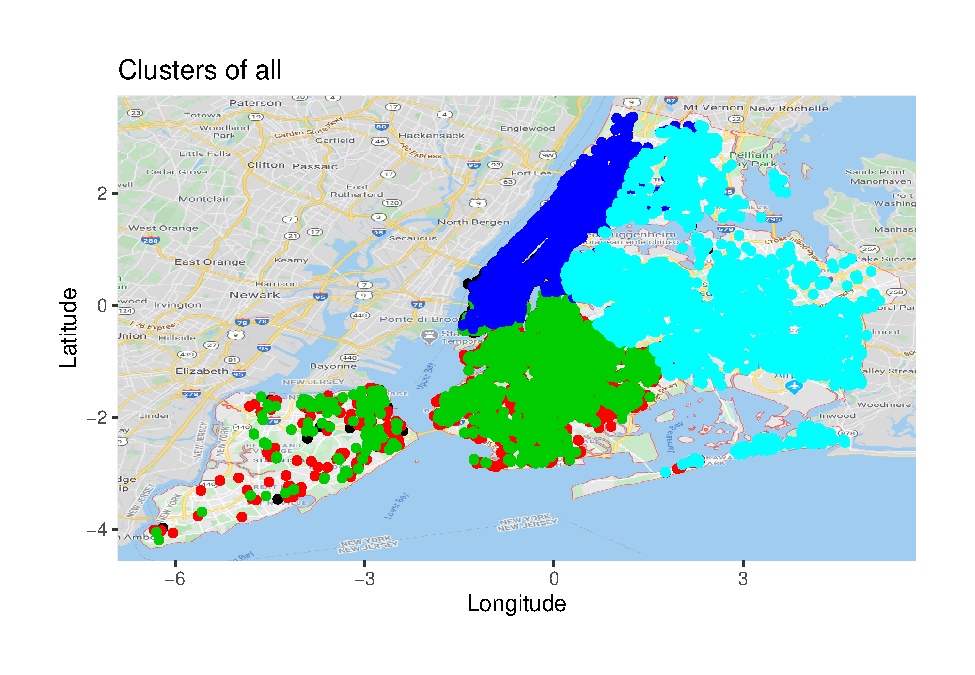
\includegraphics{unsupervised_files/figure-latex/unnamed-chunk-19-1.pdf}

\begin{Shaded}
\begin{Highlighting}[]
\CommentTok{# Contribution to the first dimension}
\KeywordTok{fviz_contrib}\NormalTok{(res.famd, }\StringTok{"var"}\NormalTok{, }\DataTypeTok{axes =} \DecValTok{1}\NormalTok{)}
\end{Highlighting}
\end{Shaded}

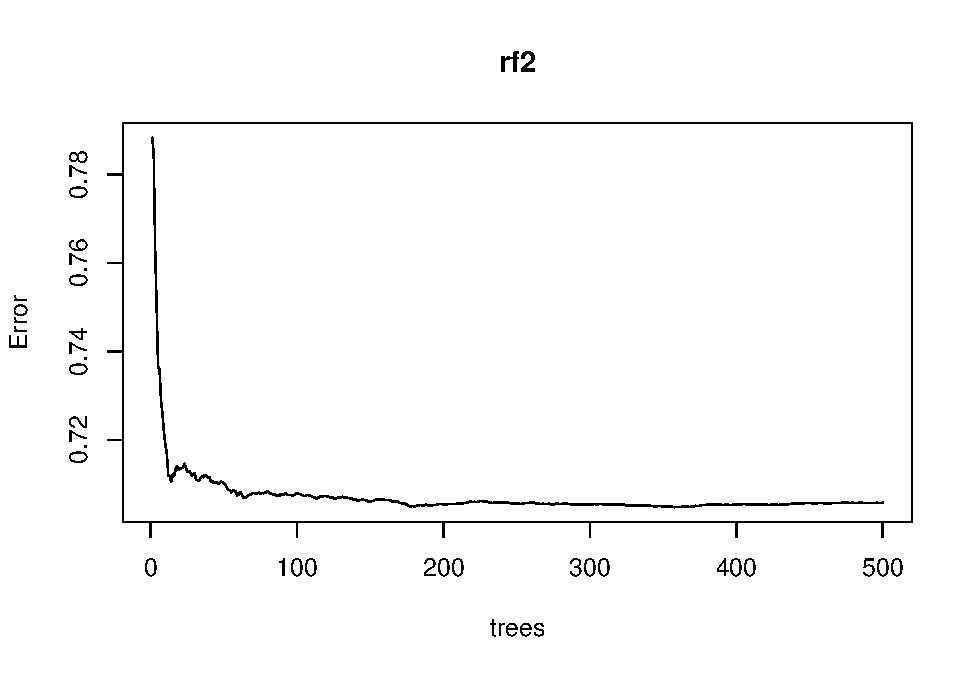
\includegraphics{unsupervised_files/figure-latex/unnamed-chunk-19-2.pdf}

\begin{Shaded}
\begin{Highlighting}[]
\CommentTok{# Contribution to the second dimension}
\KeywordTok{fviz_contrib}\NormalTok{(res.famd, }\StringTok{"var"}\NormalTok{, }\DataTypeTok{axes =} \DecValTok{2}\NormalTok{)}
\end{Highlighting}
\end{Shaded}

\includegraphics{unsupervised_files/figure-latex/unnamed-chunk-19-3.pdf}

\begin{Shaded}
\begin{Highlighting}[]
\CommentTok{# Contribution to the third dimension}
\KeywordTok{fviz_contrib}\NormalTok{(res.famd, }\StringTok{"var"}\NormalTok{, }\DataTypeTok{axes =} \DecValTok{3}\NormalTok{)}
\end{Highlighting}
\end{Shaded}

\includegraphics{unsupervised_files/figure-latex/unnamed-chunk-19-4.pdf}

\begin{Shaded}
\begin{Highlighting}[]
\CommentTok{# Contribution to the forth dimension}
\KeywordTok{fviz_contrib}\NormalTok{(res.famd, }\StringTok{"var"}\NormalTok{, }\DataTypeTok{axes =} \DecValTok{4}\NormalTok{)}
\end{Highlighting}
\end{Shaded}

\includegraphics{unsupervised_files/figure-latex/unnamed-chunk-19-5.pdf}

\begin{Shaded}
\begin{Highlighting}[]
\CommentTok{# Contribution to the fifth dimension}
\KeywordTok{fviz_contrib}\NormalTok{(res.famd, }\StringTok{"var"}\NormalTok{, }\DataTypeTok{axes =} \DecValTok{5}\NormalTok{)}
\end{Highlighting}
\end{Shaded}

\includegraphics{unsupervised_files/figure-latex/unnamed-chunk-19-6.pdf}

\begin{Shaded}
\begin{Highlighting}[]
\CommentTok{# Contribution to the sixth dimension}
\KeywordTok{fviz_contrib}\NormalTok{(res.famd, }\StringTok{"var"}\NormalTok{, }\DataTypeTok{axes =} \DecValTok{6}\NormalTok{)}
\end{Highlighting}
\end{Shaded}

\includegraphics{unsupervised_files/figure-latex/unnamed-chunk-19-7.pdf}

\begin{Shaded}
\begin{Highlighting}[]
\CommentTok{# Contribution to the seventh dimension}
\KeywordTok{fviz_contrib}\NormalTok{(res.famd, }\StringTok{"var"}\NormalTok{, }\DataTypeTok{axes =} \DecValTok{7}\NormalTok{)}
\end{Highlighting}
\end{Shaded}

\includegraphics{unsupervised_files/figure-latex/unnamed-chunk-19-8.pdf}

\begin{Shaded}
\begin{Highlighting}[]
\CommentTok{# Contribution to the eighth dimension}
\KeywordTok{fviz_contrib}\NormalTok{(res.famd, }\StringTok{"var"}\NormalTok{, }\DataTypeTok{axes =} \DecValTok{8}\NormalTok{)}
\end{Highlighting}
\end{Shaded}

\includegraphics{unsupervised_files/figure-latex/unnamed-chunk-19-9.pdf}

\hypertarget{pcamixdata}{%
\section{PCAmixdata}\label{pcamixdata}}

\begin{Shaded}
\begin{Highlighting}[]
\CommentTok{## Import library}
\KeywordTok{library}\NormalTok{(PCAmixdata)}
\end{Highlighting}
\end{Shaded}

\begin{verbatim}
## Warning: package 'PCAmixdata' was built under R version 3.6.3
\end{verbatim}

\begin{Shaded}
\begin{Highlighting}[]
\CommentTok{## Split mixed dataset into quantitative and qualitative variables}
\CommentTok{## For now excluding the target variable "Churn", which will be added later as a supplementary variable}
\NormalTok{split <-}\StringTok{ }\KeywordTok{splitmix}\NormalTok{(dataset[}\DecValTok{1}\OperatorTok{:}\DecValTok{5}\NormalTok{])  }

\CommentTok{## PCA}
\NormalTok{res.pcamix <-}\StringTok{ }\KeywordTok{PCAmix}\NormalTok{(}\DataTypeTok{X.quanti=}\NormalTok{split}\OperatorTok{$}\NormalTok{X.quanti,  }
                     \DataTypeTok{X.quali=}\NormalTok{split}\OperatorTok{$}\NormalTok{X.quali, }
                     \DataTypeTok{rename.level=}\OtherTok{TRUE}\NormalTok{, }
                     \DataTypeTok{graph=}\OtherTok{FALSE}\NormalTok{, }
                     \DataTypeTok{ndim=}\DecValTok{25}\NormalTok{)}

\NormalTok{res.pcamix}
\end{Highlighting}
\end{Shaded}

\begin{verbatim}
## 
## Call:
## PCAmix(X.quanti = split$X.quanti, X.quali = split$X.quali, ndim = 25,     rename.level = TRUE, graph = FALSE)
## 
## Method = Principal Component of mixed data (PCAmix)
## 
## 
## "name" "description"
## "$eig" "eigenvalues of the principal components (PC) "
## "$ind" "results for the individuals (coord,contrib,cos2)"
## "$quanti" "results for the quantitative variables (coord,contrib,cos2)"
## "$levels" "results for the levels of the qualitative variables (coord,contrib,cos2)"
## "$quali" "results for the qualitative variables (contrib,relative contrib)"
## "$sqload" "squared loadings"
## "$coef" "coef of the linear combinations defining the PC"
\end{verbatim}

\begin{Shaded}
\begin{Highlighting}[]
\CommentTok{## Inspect principal components}
\NormalTok{res.pcamix}\OperatorTok{$}\NormalTok{eig}
\end{Highlighting}
\end{Shaded}

\begin{verbatim}
##       Eigenvalue Proportion Cumulative
## dim 1  1.9083514  21.203905   21.20390
## dim 2  1.7965387  19.961541   41.16545
## dim 3  1.1478319  12.753688   53.91913
## dim 4  1.0050505  11.167228   65.08636
## dim 5  0.9953729  11.059699   76.14606
## dim 6  0.9550886  10.612095   86.75815
## dim 7  0.7416724   8.240804   94.99896
## dim 8  0.2731634   3.035149   98.03411
## dim 9  0.1769303   1.965892  100.00000
\end{verbatim}

\begin{Shaded}
\begin{Highlighting}[]
\CommentTok{# Use Scree Diagram to select the components:}
\KeywordTok{plot}\NormalTok{(res.pcamix}\OperatorTok{$}\NormalTok{eig, }\DataTypeTok{type=}\StringTok{"b"}\NormalTok{, }\DataTypeTok{main=}\StringTok{"Scree Diagram"}\NormalTok{, }\DataTypeTok{xlab=}\StringTok{"Number of Component"}\NormalTok{, }\DataTypeTok{ylab=}\StringTok{"Eigenvalues"}\NormalTok{)}
\KeywordTok{abline}\NormalTok{(}\DataTypeTok{h=}\DecValTok{1}\NormalTok{, }\DataTypeTok{lwd=}\DecValTok{3}\NormalTok{, }\DataTypeTok{col=}\StringTok{"red"}\NormalTok{)}
\end{Highlighting}
\end{Shaded}

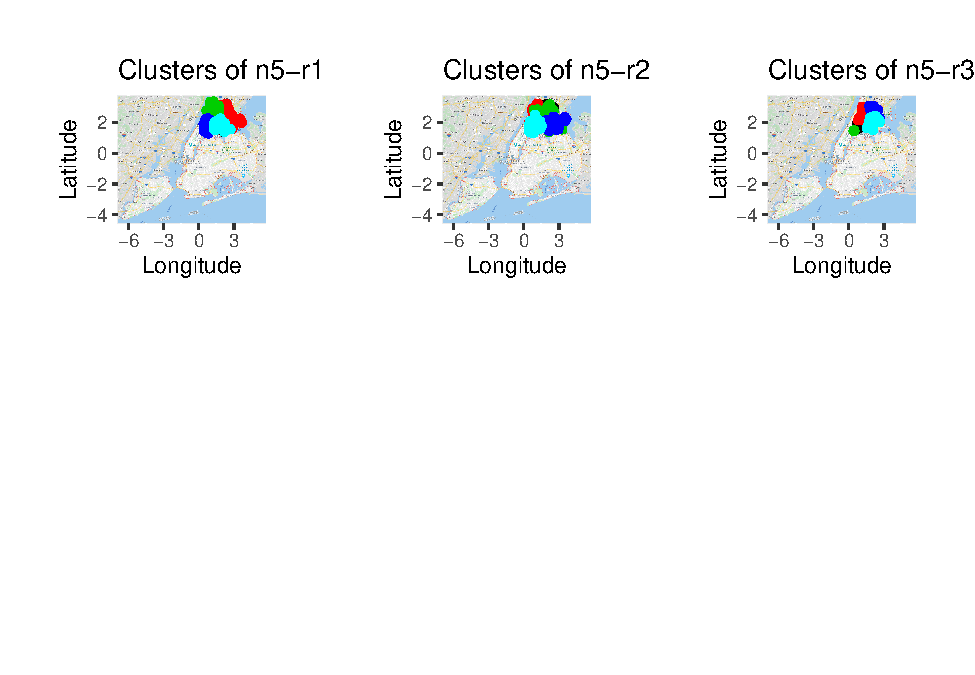
\includegraphics{unsupervised_files/figure-latex/unnamed-chunk-23-1.pdf}

\hypertarget{hierarchical-cluster-analysis}{%
\section{Hierarchical Cluster
Analysis}\label{hierarchical-cluster-analysis}}

\begin{Shaded}
\begin{Highlighting}[]
\KeywordTok{library}\NormalTok{(cluster)    }\CommentTok{# clustering algorithms}
\KeywordTok{library}\NormalTok{(dendextend) }\CommentTok{# for comparing two dendrograms}
\end{Highlighting}
\end{Shaded}

\begin{verbatim}
## Warning: package 'dendextend' was built under R version 3.6.3
\end{verbatim}

\begin{verbatim}
## 
## ---------------------
## Welcome to dendextend version 1.13.4
## Type citation('dendextend') for how to cite the package.
## 
## Type browseVignettes(package = 'dendextend') for the package vignette.
## The github page is: https://github.com/talgalili/dendextend/
## 
## Suggestions and bug-reports can be submitted at: https://github.com/talgalili/dendextend/issues
## Or contact: <tal.galili@gmail.com>
## 
##  To suppress this message use:  suppressPackageStartupMessages(library(dendextend))
## ---------------------
\end{verbatim}

\begin{verbatim}
## 
## Attaching package: 'dendextend'
\end{verbatim}

\begin{verbatim}
## The following object is masked from 'package:stats':
## 
##     cutree
\end{verbatim}

\begin{Shaded}
\begin{Highlighting}[]
\NormalTok{reduced <-}\StringTok{ }\NormalTok{dataset[ }\KeywordTok{sample}\NormalTok{(}\DecValTok{1}\OperatorTok{:}\KeywordTok{nrow}\NormalTok{(dataset), }\KeywordTok{nrow}\NormalTok{(dataset)}\OperatorTok{/}\DecValTok{10}\NormalTok{ ) , ]}
\NormalTok{d <-}\StringTok{ }\KeywordTok{dist}\NormalTok{(reduced, }\DataTypeTok{method =} \StringTok{"euclidean"}\NormalTok{)}


\CommentTok{# Hierarchical clustering using Complete Linkage}
\NormalTok{hc1 <-}\StringTok{ }\KeywordTok{hclust}\NormalTok{(d, }\DataTypeTok{method =} \StringTok{"complete"}\NormalTok{ )}

\CommentTok{# Plot the obtained dendrogram}
\KeywordTok{plot}\NormalTok{(hc1, }\DataTypeTok{cex =} \FloatTok{0.6}\NormalTok{, }\DataTypeTok{hang =} \DecValTok{-1}\NormalTok{)}
\end{Highlighting}
\end{Shaded}

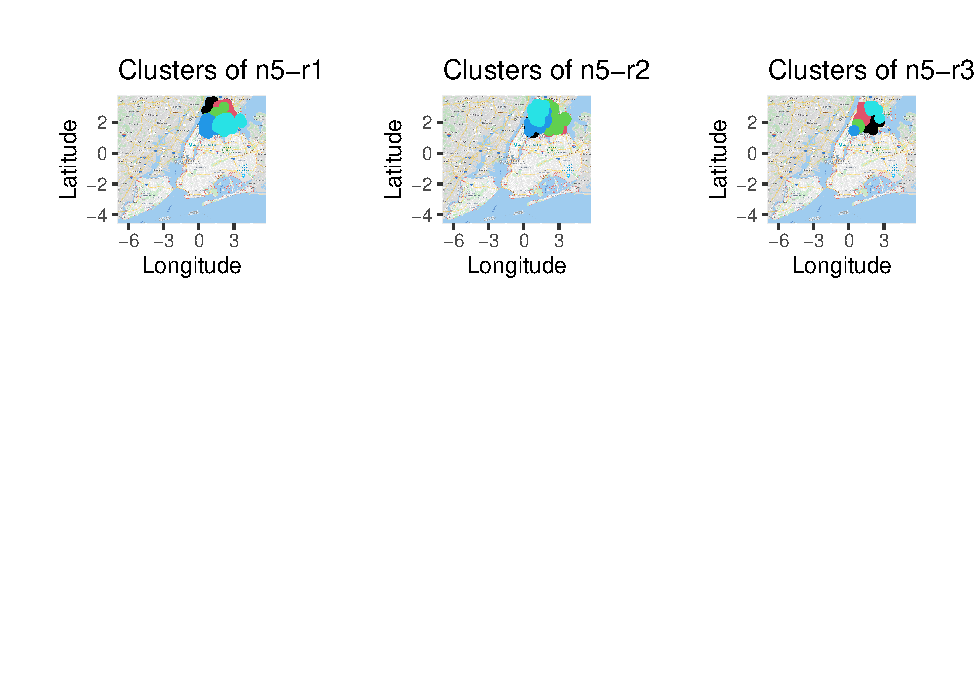
\includegraphics{unsupervised_files/figure-latex/unnamed-chunk-25-1.pdf}

\begin{Shaded}
\begin{Highlighting}[]
\CommentTok{# methods to assess}
\NormalTok{m <-}\StringTok{ }\KeywordTok{c}\NormalTok{( }\StringTok{"average"}\NormalTok{, }\StringTok{"single"}\NormalTok{, }\StringTok{"complete"}\NormalTok{, }\StringTok{"ward"}\NormalTok{)}
\KeywordTok{names}\NormalTok{(m) <-}\StringTok{ }\KeywordTok{c}\NormalTok{( }\StringTok{"average"}\NormalTok{, }\StringTok{"single"}\NormalTok{, }\StringTok{"complete"}\NormalTok{, }\StringTok{"ward"}\NormalTok{)}

\CommentTok{# function to compute coefficient}
\NormalTok{ac <-}\StringTok{ }\ControlFlowTok{function}\NormalTok{(x) \{}
  \KeywordTok{agnes}\NormalTok{(reduced, }\DataTypeTok{method =}\NormalTok{ x)}\OperatorTok{$}\NormalTok{ac}
\NormalTok{\}}

\KeywordTok{library}\NormalTok{(purrr)}
\KeywordTok{map_dbl}\NormalTok{(m, ac)}
\end{Highlighting}
\end{Shaded}

\begin{verbatim}
##   average    single  complete      ward 
## 0.9972251 0.9953447 0.9971935 0.9987706
\end{verbatim}

\begin{Shaded}
\begin{Highlighting}[]
\NormalTok{hc3 <-}\StringTok{ }\KeywordTok{agnes}\NormalTok{(reduced, }\DataTypeTok{method =} \StringTok{"ward"}\NormalTok{)}
\KeywordTok{pltree}\NormalTok{(hc3, }\DataTypeTok{cex =} \FloatTok{0.6}\NormalTok{, }\DataTypeTok{hang =} \DecValTok{-1}\NormalTok{, }\DataTypeTok{main =} \StringTok{"Dendrogram of agnes"}\NormalTok{) }
\end{Highlighting}
\end{Shaded}

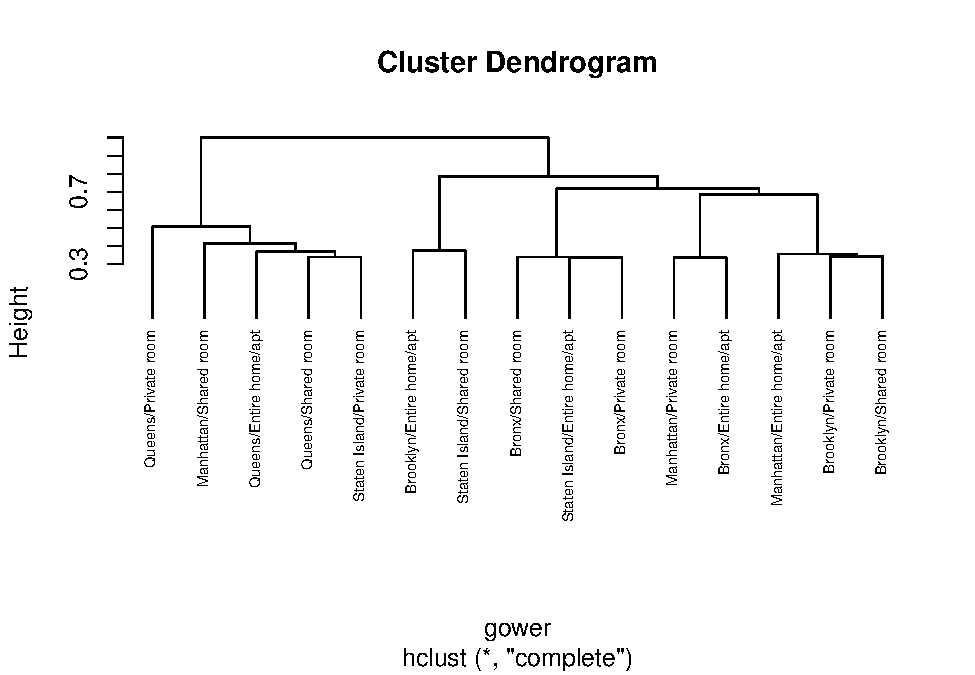
\includegraphics{unsupervised_files/figure-latex/unnamed-chunk-27-1.pdf}

\hypertarget{clust-mix-type}{%
\section{Clust miX type}\label{clust-mix-type}}

k-prototypes in RAn implementation of the k-prototypes algorithm is
given by the function

kproto(x, k, lambda = NULL, iter.max = 100, nstart = 1, na.rm = TRUE)

where •x is a data frame with both numeric and factor variables. As
opposed to other existing Rpackages, the factor variables do not need to
be preprocessed in advance and the order of thevariables does not
matter. •k is the number of clusters which has to be pre-specified.
Alternatively, it can also be a vectorof observation indices or a data
frame of prototypes with the same columns asx. If ever atthe
initialization or during the iteration process identical prototypes do
occur, the number ofclusters will be reduced accordingly.

•lambda\textgreater0 is a real valued parameter that controls the trade
off between Euclidean distancefor numeric variables and simple matching
distance for factor variables for cluster assignment.If noλis specified
the parameter is set automatically based on the data and a heuristic
usingthe functionlambdaest(). Alternatively, a vector of
lengthncol(x)can be passed tolambda(cf.Section on Extensions to the
original algorithm).

•iter.maxsets the maximum number of iterations, just as inkmeans(). The
algorithm may stopprior toiter.maxif no observations swap clusters.

•nstartmay be set to a value\textgreater1 to run k-prototypes multiple
times. Similar to k-means, theresult of k-prototypes depends on its
initialization. Ifnstart\textgreater1, the best solution (i.e.~the
onethat minimizesE) is returned.

•Generally, the algorithm can deal with missing data but as a defaultNAs
are removed byna.rm= TRUE

\begin{Shaded}
\begin{Highlighting}[]
\KeywordTok{library}\NormalTok{(clustMixType)}
\end{Highlighting}
\end{Shaded}

\begin{verbatim}
## Warning: package 'clustMixType' was built under R version 3.6.3
\end{verbatim}

\begin{Shaded}
\begin{Highlighting}[]
\NormalTok{kp =}\StringTok{ }\KeywordTok{kproto}\NormalTok{(dataset,}\DecValTok{5}\NormalTok{)}
\end{Highlighting}
\end{Shaded}

\begin{verbatim}
## # NAs in variables:
## neighbourhood_group            latitude           longitude           room_type 
##                   0                   0                   0                   0 
##               price 
##                   0 
## 0 observation(s) with NAs.
## 
## Estimated lambda: 1.751941
\end{verbatim}

\begin{Shaded}
\begin{Highlighting}[]
\NormalTok{kp }
\end{Highlighting}
\end{Shaded}

\begin{verbatim}
## Numeric predictors: 3 
## Categorical predictors: 2 
## Lambda: 1.751941 
## 
## Number of Clusters: 5 
## Cluster sizes: 7878 114 5364 16565 18974 
## Within cluster error: 11397.74 9345.631 15618.47 26432.3 30432.57 
## 
## Cluster prototypes:
##   neighbourhood_group    latitude    longitude room_type      price
## 1                   2  1.50386444  0.146224465         1 -0.2358076
## 2                   2  0.12878738 -0.508329735         2 14.7620392
## 3                   3  0.03222822  1.878923383         1 -0.2596570
## 4                   2  0.24905671 -0.667719629         2  0.3222203
## 5                   1 -0.85172459 -0.005891015         1 -0.1986908
\end{verbatim}

\begin{Shaded}
\begin{Highlighting}[]
\KeywordTok{summary}\NormalTok{(kp)}
\end{Highlighting}
\end{Shaded}

\begin{verbatim}
## neighbourhood_group 
##        
## cluster     1     2     3     4     5
##       1 0.000 0.867 0.012 0.000 0.121
##       2 0.219 0.719 0.044 0.009 0.009
##       3 0.018 0.000 0.956 0.000 0.026
##       4 0.077 0.890 0.024 0.009 0.000
##       5 0.986 0.000 0.002 0.012 0.000
## 
## -----------------------------------------------------------------
## latitude 
##        Min.    1st Qu.     Median        Mean    3rd Qu.      Max.
## 1  0.193125  1.1469564  1.4926830  1.50386444  1.8435902 3.3763223
## 2 -2.664931 -0.2424603  0.1314159  0.12878738  0.7171018 2.8931028
## 3 -2.998141 -0.4437712  0.2545589  0.03222822  0.5621415 2.5217481
## 4 -4.081030 -0.1070763  0.2055951  0.24905671  0.6127099 1.9578391
## 5 -4.202431 -1.0755327 -0.7819332 -0.85172459 -0.5052511 0.3244286
## 
## -----------------------------------------------------------------
## longitude 
##         Min.    1st Qu.     Median         Mean    3rd Qu.      Max.
## 1 -0.9981292 -0.1192759  0.1291169  0.146224465  0.3009228 2.6065451
## 2 -3.1442948 -0.9795512 -0.6625335 -0.508329735 -0.2576089 3.9318121
## 3  0.1304168  0.8738619  1.5712683  1.878923383  2.7664893 5.1819005
## 4 -6.3316952 -0.9424493 -0.7158302 -0.667719629 -0.4094827 0.8718037
## 5 -6.2976807 -0.2515426  0.0279399 -0.005891015  0.3758306 1.7067848
## 
## -----------------------------------------------------------------
## room_type 
##        
## cluster     1     2     3
##       1 0.737 0.229 0.033
##       2 0.175 0.825 0.000
##       3 0.626 0.336 0.038
##       4 0.171 0.812 0.017
##       5 0.543 0.435 0.022
## 
## -----------------------------------------------------------------
## price 
##         Min.     1st Qu.     Median       Mean     3rd Qu.      Max.
## 1 -0.6359277 -0.38608818 -0.2819884 -0.2358076 -0.15706863  3.528064
## 2  7.6004481  7.82738569 11.6270282 14.7620392 16.85283798 41.003991
## 3 -0.5942878 -0.42772810 -0.3444483 -0.2596570 -0.21952851  5.610060
## 4 -0.6359277 -0.09460876  0.1427388  0.3222203  0.44671018  7.275657
## 5 -0.6359277 -0.38608818 -0.2778244 -0.1986908 -0.09460876  3.944463
## 
## -----------------------------------------------------------------
\end{verbatim}

\begin{Shaded}
\begin{Highlighting}[]
\KeywordTok{library}\NormalTok{(wesanderson)}
\KeywordTok{par}\NormalTok{(}\DataTypeTok{mfrow=}\KeywordTok{c}\NormalTok{(}\DecValTok{2}\NormalTok{,}\DecValTok{2}\NormalTok{))}
\KeywordTok{clprofiles}\NormalTok{(kp, dataset, }\DataTypeTok{col =} \KeywordTok{wes_palette}\NormalTok{(}\StringTok{"Royal1"}\NormalTok{,}\DecValTok{5}\NormalTok{, }\DataTypeTok{type =} \StringTok{"continuous"}\NormalTok{))  }
\end{Highlighting}
\end{Shaded}

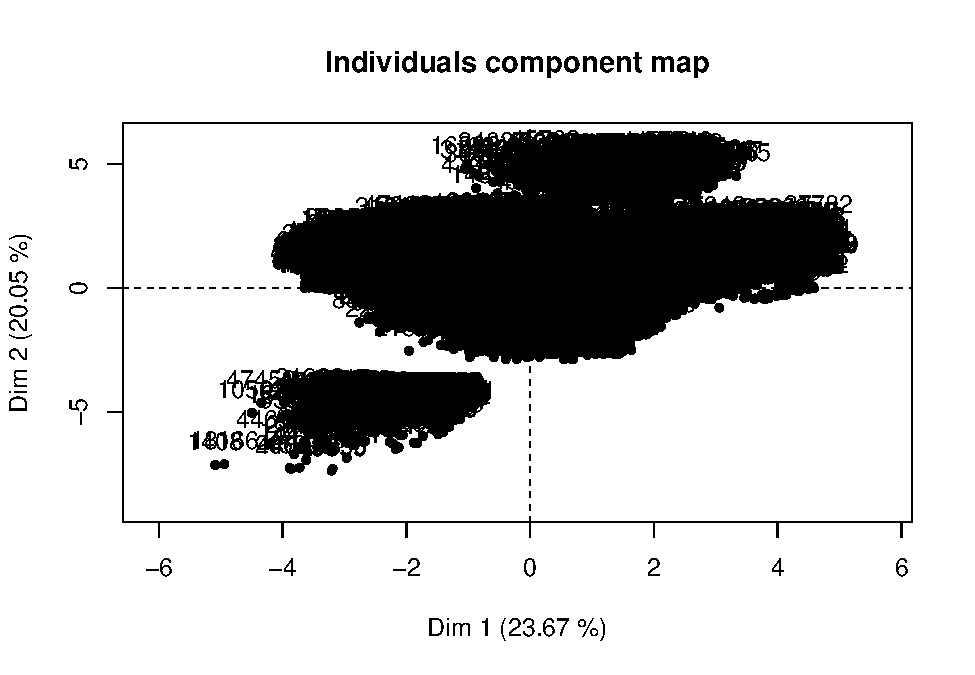
\includegraphics{unsupervised_files/figure-latex/unnamed-chunk-29-1.pdf}
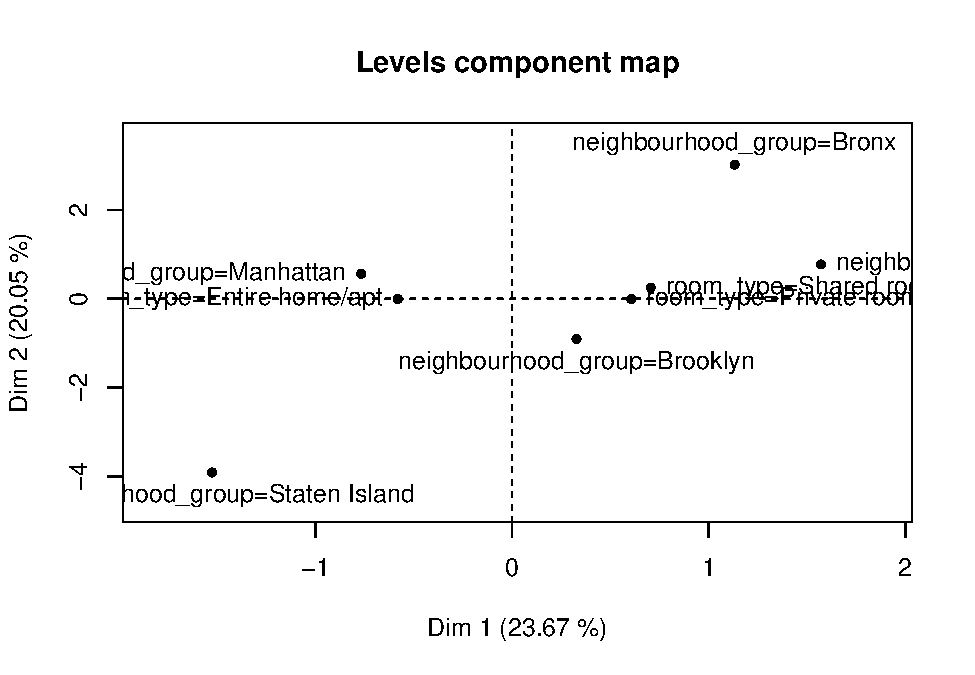
\includegraphics{unsupervised_files/figure-latex/unnamed-chunk-29-2.pdf}

\begin{Shaded}
\begin{Highlighting}[]
\NormalTok{Es =}\StringTok{ }\KeywordTok{numeric}\NormalTok{(}\DecValTok{10}\NormalTok{)}
\ControlFlowTok{for}\NormalTok{(i }\ControlFlowTok{in} \DecValTok{1}\OperatorTok{:}\DecValTok{10}\NormalTok{)}
\NormalTok{  \{}
\NormalTok{    kpres <-}\StringTok{ }\KeywordTok{kproto}\NormalTok{(dataset, }\DataTypeTok{k =}\NormalTok{ i, }\DataTypeTok{nstart =} \DecValTok{5}\NormalTok{)}
\NormalTok{    Es[i] <-}\StringTok{ }\NormalTok{kpres}\OperatorTok{$}\NormalTok{tot.withinss}
\NormalTok{  \}}
\end{Highlighting}
\end{Shaded}

\begin{verbatim}
## # NAs in variables:
## neighbourhood_group            latitude           longitude           room_type 
##                   0                   0                   0                   0 
##               price 
##                   0 
## 0 observation(s) with NAs.
## 
## Estimated lambda: 1.751941 
## 
## # NAs in variables:
## neighbourhood_group            latitude           longitude           room_type 
##                   0                   0                   0                   0 
##               price 
##                   0 
## 0 observation(s) with NAs.
## 
## # NAs in variables:
## neighbourhood_group            latitude           longitude           room_type 
##                   0                   0                   0                   0 
##               price 
##                   0 
## 0 observation(s) with NAs.
## 
## # NAs in variables:
## neighbourhood_group            latitude           longitude           room_type 
##                   0                   0                   0                   0 
##               price 
##                   0 
## 0 observation(s) with NAs.
## 
## # NAs in variables:
## neighbourhood_group            latitude           longitude           room_type 
##                   0                   0                   0                   0 
##               price 
##                   0 
## 0 observation(s) with NAs.
## 
## # NAs in variables:
## neighbourhood_group            latitude           longitude           room_type 
##                   0                   0                   0                   0 
##               price 
##                   0 
## 0 observation(s) with NAs.
## 
## Estimated lambda: 1.751941 
## 
## # NAs in variables:
## neighbourhood_group            latitude           longitude           room_type 
##                   0                   0                   0                   0 
##               price 
##                   0 
## 0 observation(s) with NAs.
## 
## # NAs in variables:
## neighbourhood_group            latitude           longitude           room_type 
##                   0                   0                   0                   0 
##               price 
##                   0 
## 0 observation(s) with NAs.
## 
## # NAs in variables:
## neighbourhood_group            latitude           longitude           room_type 
##                   0                   0                   0                   0 
##               price 
##                   0 
## 0 observation(s) with NAs.
## 
## # NAs in variables:
## neighbourhood_group            latitude           longitude           room_type 
##                   0                   0                   0                   0 
##               price 
##                   0 
## 0 observation(s) with NAs.
## 
## # NAs in variables:
## neighbourhood_group            latitude           longitude           room_type 
##                   0                   0                   0                   0 
##               price 
##                   0 
## 0 observation(s) with NAs.
## 
## Estimated lambda: 1.751941 
## 
## # NAs in variables:
## neighbourhood_group            latitude           longitude           room_type 
##                   0                   0                   0                   0 
##               price 
##                   0 
## 0 observation(s) with NAs.
## 
## # NAs in variables:
## neighbourhood_group            latitude           longitude           room_type 
##                   0                   0                   0                   0 
##               price 
##                   0 
## 0 observation(s) with NAs.
## 
## # NAs in variables:
## neighbourhood_group            latitude           longitude           room_type 
##                   0                   0                   0                   0 
##               price 
##                   0 
## 0 observation(s) with NAs.
## 
## # NAs in variables:
## neighbourhood_group            latitude           longitude           room_type 
##                   0                   0                   0                   0 
##               price 
##                   0 
## 0 observation(s) with NAs.
## 
## # NAs in variables:
## neighbourhood_group            latitude           longitude           room_type 
##                   0                   0                   0                   0 
##               price 
##                   0 
## 0 observation(s) with NAs.
## 
## Estimated lambda: 1.751941 
## 
## # NAs in variables:
## neighbourhood_group            latitude           longitude           room_type 
##                   0                   0                   0                   0 
##               price 
##                   0 
## 0 observation(s) with NAs.
## 
## # NAs in variables:
## neighbourhood_group            latitude           longitude           room_type 
##                   0                   0                   0                   0 
##               price 
##                   0 
## 0 observation(s) with NAs.
## 
## # NAs in variables:
## neighbourhood_group            latitude           longitude           room_type 
##                   0                   0                   0                   0 
##               price 
##                   0 
## 0 observation(s) with NAs.
## 
## # NAs in variables:
## neighbourhood_group            latitude           longitude           room_type 
##                   0                   0                   0                   0 
##               price 
##                   0 
## 0 observation(s) with NAs.
## 
## # NAs in variables:
## neighbourhood_group            latitude           longitude           room_type 
##                   0                   0                   0                   0 
##               price 
##                   0 
## 0 observation(s) with NAs.
## 
## Estimated lambda: 1.751941 
## 
## # NAs in variables:
## neighbourhood_group            latitude           longitude           room_type 
##                   0                   0                   0                   0 
##               price 
##                   0 
## 0 observation(s) with NAs.
## 
## # NAs in variables:
## neighbourhood_group            latitude           longitude           room_type 
##                   0                   0                   0                   0 
##               price 
##                   0 
## 0 observation(s) with NAs.
## 
## # NAs in variables:
## neighbourhood_group            latitude           longitude           room_type 
##                   0                   0                   0                   0 
##               price 
##                   0 
## 0 observation(s) with NAs.
## 
## # NAs in variables:
## neighbourhood_group            latitude           longitude           room_type 
##                   0                   0                   0                   0 
##               price 
##                   0 
## 0 observation(s) with NAs.
## 
## # NAs in variables:
## neighbourhood_group            latitude           longitude           room_type 
##                   0                   0                   0                   0 
##               price 
##                   0 
## 0 observation(s) with NAs.
## 
## Estimated lambda: 1.751941 
## 
## # NAs in variables:
## neighbourhood_group            latitude           longitude           room_type 
##                   0                   0                   0                   0 
##               price 
##                   0 
## 0 observation(s) with NAs.
## 
## # NAs in variables:
## neighbourhood_group            latitude           longitude           room_type 
##                   0                   0                   0                   0 
##               price 
##                   0 
## 0 observation(s) with NAs.
## 
## # NAs in variables:
## neighbourhood_group            latitude           longitude           room_type 
##                   0                   0                   0                   0 
##               price 
##                   0 
## 0 observation(s) with NAs.
## 
## # NAs in variables:
## neighbourhood_group            latitude           longitude           room_type 
##                   0                   0                   0                   0 
##               price 
##                   0 
## 0 observation(s) with NAs.
## 
## # NAs in variables:
## neighbourhood_group            latitude           longitude           room_type 
##                   0                   0                   0                   0 
##               price 
##                   0 
## 0 observation(s) with NAs.
## 
## Estimated lambda: 1.751941 
## 
## # NAs in variables:
## neighbourhood_group            latitude           longitude           room_type 
##                   0                   0                   0                   0 
##               price 
##                   0 
## 0 observation(s) with NAs.
## 
## # NAs in variables:
## neighbourhood_group            latitude           longitude           room_type 
##                   0                   0                   0                   0 
##               price 
##                   0 
## 0 observation(s) with NAs.
## 
## # NAs in variables:
## neighbourhood_group            latitude           longitude           room_type 
##                   0                   0                   0                   0 
##               price 
##                   0 
## 0 observation(s) with NAs.
## 
## # NAs in variables:
## neighbourhood_group            latitude           longitude           room_type 
##                   0                   0                   0                   0 
##               price 
##                   0 
## 0 observation(s) with NAs.
## 
## # NAs in variables:
## neighbourhood_group            latitude           longitude           room_type 
##                   0                   0                   0                   0 
##               price 
##                   0 
## 0 observation(s) with NAs.
## 
## Estimated lambda: 1.751941 
## 
## # NAs in variables:
## neighbourhood_group            latitude           longitude           room_type 
##                   0                   0                   0                   0 
##               price 
##                   0 
## 0 observation(s) with NAs.
## 
## # NAs in variables:
## neighbourhood_group            latitude           longitude           room_type 
##                   0                   0                   0                   0 
##               price 
##                   0 
## 0 observation(s) with NAs.
## 
## # NAs in variables:
## neighbourhood_group            latitude           longitude           room_type 
##                   0                   0                   0                   0 
##               price 
##                   0 
## 0 observation(s) with NAs.
## 
## # NAs in variables:
## neighbourhood_group            latitude           longitude           room_type 
##                   0                   0                   0                   0 
##               price 
##                   0 
## 0 observation(s) with NAs.
## 
## # NAs in variables:
## neighbourhood_group            latitude           longitude           room_type 
##                   0                   0                   0                   0 
##               price 
##                   0 
## 0 observation(s) with NAs.
## 
## Estimated lambda: 1.751941 
## 
## # NAs in variables:
## neighbourhood_group            latitude           longitude           room_type 
##                   0                   0                   0                   0 
##               price 
##                   0 
## 0 observation(s) with NAs.
## 
## # NAs in variables:
## neighbourhood_group            latitude           longitude           room_type 
##                   0                   0                   0                   0 
##               price 
##                   0 
## 0 observation(s) with NAs.
## 
## # NAs in variables:
## neighbourhood_group            latitude           longitude           room_type 
##                   0                   0                   0                   0 
##               price 
##                   0 
## 0 observation(s) with NAs.
## 
## # NAs in variables:
## neighbourhood_group            latitude           longitude           room_type 
##                   0                   0                   0                   0 
##               price 
##                   0 
## 0 observation(s) with NAs.
## 
## # NAs in variables:
## neighbourhood_group            latitude           longitude           room_type 
##                   0                   0                   0                   0 
##               price 
##                   0 
## 0 observation(s) with NAs.
## 
## Estimated lambda: 1.751941 
## 
## # NAs in variables:
## neighbourhood_group            latitude           longitude           room_type 
##                   0                   0                   0                   0 
##               price 
##                   0 
## 0 observation(s) with NAs.
## 
## # NAs in variables:
## neighbourhood_group            latitude           longitude           room_type 
##                   0                   0                   0                   0 
##               price 
##                   0 
## 0 observation(s) with NAs.
## 
## # NAs in variables:
## neighbourhood_group            latitude           longitude           room_type 
##                   0                   0                   0                   0 
##               price 
##                   0 
## 0 observation(s) with NAs.
## 
## # NAs in variables:
## neighbourhood_group            latitude           longitude           room_type 
##                   0                   0                   0                   0 
##               price 
##                   0 
## 0 observation(s) with NAs.
\end{verbatim}

\begin{Shaded}
\begin{Highlighting}[]
\KeywordTok{plot}\NormalTok{(}\DecValTok{1}\OperatorTok{:}\DecValTok{10}\NormalTok{, Es, }\DataTypeTok{type =} \StringTok{"b"}\NormalTok{, }\DataTypeTok{ylab =} \StringTok{"Objective Function"}\NormalTok{, }\DataTypeTok{xlab =} \StringTok{"# Clusters"}\NormalTok{,}\DataTypeTok{main =} \StringTok{"Scree Plot"}\NormalTok{) }
\end{Highlighting}
\end{Shaded}

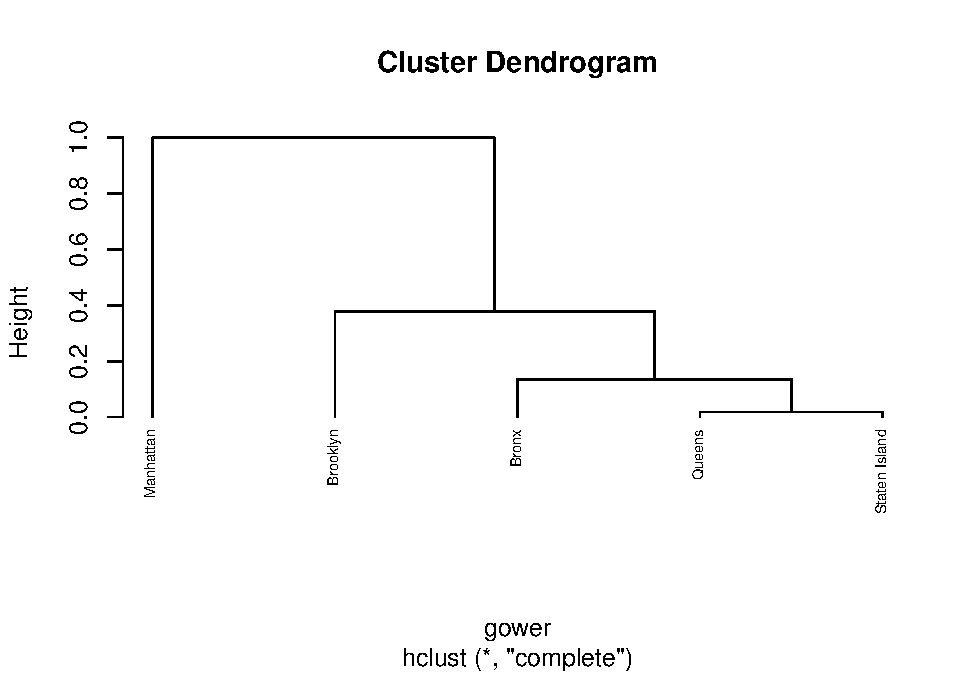
\includegraphics{unsupervised_files/figure-latex/unnamed-chunk-30-1.pdf}

\end{document}
